\documentclass{article}

% Language setting
% Replace `english' with e.g. `spanish' to change the document language
\usepackage[english]{babel}
\usepackage[utf8]{inputenc}
\usepackage[T1]{fontenc}

\usepackage[letterpaper,top=2cm,bottom=5cm,left=3cm,right=3cm,marginparwidth=1.75cm]{geometry}

% Useful packages
\usepackage{amsmath}
\usepackage{graphicx}
\usepackage[colorlinks=true, allcolors=blue]{hyperref}
\usepackage{amssymb}
\usepackage{fancyhdr}
\usepackage{lipsum} % Para generar texto de ejemplo
\usepackage{multicol}
\usepackage{tikz}
\usetikzlibrary{arrows.meta, positioning}
\usepackage{booktabs}
\usepackage{array}
\usepackage{float}
\pagestyle{fancy}

\fancyhf{} % Limpiar encabezado y pie de página por defecto
\setlength{\headheight}{70pt} % Ajuste del tamaño del encabezado

% Definición del encabezado
\fancyhead[C]{%
    \begin{minipage}[c]{1.5cm}
        
\includegraphics[width=1.5cm]{imagenes/uta.png}
    \end{minipage}%
    \hfill  % <--- SIN EL SIGNO % (descomentado)
    \begin{minipage}[c]{10cm}
        \centering
        \small {\textbf{UNIVERSIDAD TÉCNICA DE AMBATO}} \\[0.1cm]
        \scriptsize \textit{FACULTAD DE INGENIERÍA EN SISTEMAS ELECTRÓNICA E INDUSTRIAL} \\[0.1cm]
        \scriptsize \textbf{CARRERA SOFTWARE - INVESTIGACIÓN OPERATIVA} \\[0.1cm]
        \scriptsize \textbf{CICLO ACADÉMICO: ENERO - JULIO 2026}
        \vspace{0.2cm} % <--- Espacio entre texto y línea horizontal
    \end{minipage}%
    \hfill  % <--- SIN EL SIGNO % (descomentado)
    \begin{minipage}[c]{1.5cm}
        \centering
        
\includegraphics[width=1.5cm]{imagenes/fisei.png}
    \end{minipage}%
}

\begin{document}
\begin{center}
    {\large \textbf{INFORME DE GUÍA PRÁCTICA}} \\
\end{center}

\section{Portada}
\begin{flushleft}
\begin{tabular}{ l p{8.3cm} }
    \textbf{Tema:} & Modelo de planeación, revisión y evaluación de operaciones y gestión de proyectos. MS/Project esencial y avanzado. SW \\
    \textbf{Unidad de Organización Curricular:} & Unidad Profesional \\
    \textbf{Nivel y Paralelo:} & 5to Semestre "A" \\
    \textbf{Alumnos participante(s):} & Guatemal Avilez Bryan Stalin\\
    & \dotfill \\
    \textbf{Asignatura:} & Investigación Operativa \\
    \textbf{Docente:} & Ing. Inti Israel Becerra Loaiza, Mg. \\
\end{tabular}
\end{flushleft}

\section{Informe de guía práctica}
\subsection{Objetivos}
\subsubsection{General}
Aplicar el método de la ruta crítica (CPM) y los diagramas de Gantt en la planeación, programación y control de proyectos, como base conceptual para el uso de herramientas de gestión como MS Project.

\subsubsection{Específicos}
\begin{itemize}
    \item Construir la red de precedencias (AON) del Ejercicio 2, calcular los tiempos $ES$, $EF$, $LS$, $LF$ y las holguras total y libre, y determinar la ruta crítica.
    \item Analizar conceptualmente las holguras total y libre de una actividad crítica (Ejercicio 3) y verificarlas numéricamente con los datos de las redes resueltas.
    \item Determinar la ruta crítica de los dos proyectos (redes AOA) del Ejercicio 5 y elaborar sus respectivos diagramas de Gantt.
\end{itemize}

\subsection{Modalidad}
Presencial.

\subsection{Tiempo de duración}

Presenciales: 4 horas\\
No presenciales: 0 horas

\subsection{Instrucciones}

\begin{itemize}
    \item Revisar detenidamente la guía proporcionada y analizar la información de clase.
    \item Investigar información adicional y complementaria sobre los casos propuestos.
    \item Complementar conocimientos y aplicaciones de MS Project mediante la resolución manual de los ejercicios de redes y CPM.
\end{itemize}

\subsection{Listado de equipos, materiales y recursos}
\textbf{Listado de equipos y materiales generales empleados en la guía práctica:}
\begin{itemize}
    \item Tarea 07 y formulario de la guía práctica proporcionados por el docente.
    \item Bibliografía de Investigación de Operaciones (Taha, Palacios Figueroa, Martín, PMI).
    \item Computador con Python y editor LaTeX, empleados para verificar los cálculos del método CPM y elaborar el presente informe.
    \item Cuaderno de trabajo, lápiz, borrador y calculadora.
\end{itemize}

\textbf{TAC (Tecnologías para el Aprendizaje y Conocimiento) empleados en la guía práctica:}
\begin{itemize}
    \item[$\square$] Plataformas educativas
    \item[$\square$] Simuladores y laboratorios virtuales
    \item[$\square$] Aplicaciones educativas
    \item[$\square$] Recursos audiovisuales
    \item[$\square$] Gamificación
    \item[$\boxtimes$] Inteligencia Artificial
    \item Otros (Especifique): \underline{\hspace{5cm}}
\end{itemize}

\subsection{Actividades por desarrollar}

\begin{itemize}
    \item Revisar la guía y la Tarea 07 entregadas por el docente.
    \item Analizar los Ejercicios 2, 3 y 5 planteados.
    \item Construir las redes de actividades (AON para el Ejercicio 2 y AOA para el Ejercicio 5).
    \item Aplicar el método CPM: paso hacia adelante ($ES$, $EF$), paso hacia atrás ($LS$, $LF$) y cálculo de holguras ($TF$, $FF$).
    \item Elaborar los diagramas de Gantt de los proyectos (a) y (b) del Ejercicio 5 y determinar las rutas críticas correspondientes.
\end{itemize}

\subsection{Resultados obtenidos}

De acuerdo con la Tarea 07 de Investigación Operativa, se seleccionaron y resolvieron los Ejercicios 2, 3 y 5, aplicando el método de la ruta crítica (CPM) y la elaboración de diagramas de Gantt. A continuación se presentan los resultados obtenidos para cada ejercicio.

\subsubsection{Ejercicio 2: Red de precedencias y método CPM}

\textbf{Enunciado:} Una compañía está preparando un presupuesto para lanzar un nuevo producto. La siguiente tabla muestra las actividades asociadas y su duración. Construya la red del proyecto.

\begin{center}
\begin{tabular}{|l|c|c|}
\hline
\textbf{Actividad} & \textbf{Predecesora(s)} & \textbf{Duración (días)} \\
\hline
A: Pronosticar volumen de ventas & -- & 10 \\
B: Estudiar el mercado competitivo & -- & 7 \\
C: Diseñar artículo e instalaciones & A & 5 \\
D: Preparar el programa de producción & C & 3 \\
E: Estimar el costo de la producción & D & 2 \\
F: Fijar precio de venta & B, E & 1 \\
G: Preparar presupuesto & E, F & 14 \\
\hline
\end{tabular}
\end{center}

\textbf{Red del proyecto (diagrama de precedencias, AON):}

\begin{figure}[H]
\centering
\resizebox{0.95\textwidth}{!}{%
\begin{tikzpicture}[
  act/.style={rectangle, draw, thick, rounded corners=2pt, minimum width=1.6cm, minimum height=1.1cm, align=center, font=\small},
  >={Stealth[length=3mm]}, line width=0.8pt
]
  \node[act] (A) at (0,0)    {A\\$D=10$};
  \node[act] (C) at (2.6,0)  {C\\$D=5$};
  \node[act] (D) at (5.2,0)  {D\\$D=3$};
  \node[act] (E) at (7.8,0)  {E\\$D=2$};
  \node[act] (F) at (10.4,0) {F\\$D=1$};
  \node[act] (G) at (13.0,0) {G\\$D=14$};
  \node[act] (B) at (10.4,-2.4) {B\\$D=7$};

  \draw[->] (A) -- (C);
  \draw[->] (C) -- (D);
  \draw[->] (D) -- (E);
  \draw[->] (E) -- (F);
  \draw[->] (F) -- (G);
  \draw[->] (B) -- (F);
  \draw[->] (E) to[bend left=20] (G);
\end{tikzpicture}%
}
\caption{Red de precedencias (AON) del Ejercicio 2}
\label{fig:ej2-aon}
\end{figure}

\textbf{Análisis CPM:}

\begin{center}
\small
\begin{tabular}{|c|c|c|c|c|c|c|c|c|}
\hline
\textbf{Act.} & \textbf{Dur.} & \textbf{ES} & \textbf{EF} & \textbf{LS} & \textbf{LF} & \textbf{TF} & \textbf{FF} & \textbf{¿Crítica?} \\
\hline
A & 10 & 0  & 10 & 0  & 10 & 0  & 0  & Sí \\
B & 7  & 0  & 7  & 13 & 20 & 13 & 13 & No \\
C & 5  & 10 & 15 & 10 & 15 & 0  & 0  & Sí \\
D & 3  & 15 & 18 & 15 & 18 & 0  & 0  & Sí \\
E & 2  & 18 & 20 & 18 & 20 & 0  & 0  & Sí \\
F & 1  & 20 & 21 & 20 & 21 & 0  & 0  & Sí \\
G & 14 & 21 & 35 & 21 & 35 & 0  & 0  & Sí \\
\hline
\end{tabular}
\end{center}

\textbf{Conclusión:} La duración total del proyecto es de $T = 35$ días. La ruta crítica es \textbf{A--C--D--E--F--G} ($10+5+3+2+1+14=35$). La actividad B es la única no crítica, con holgura total $TF=13$ y holgura libre $FF=13$ días, por lo que puede iniciarse hasta 13 días después de su inicio más temprano sin retrasar el proyecto.

\subsubsection{Ejercicio 3: Holguras total y libre de una actividad crítica}

\textbf{Enunciado:} ¿Cuáles son los flotantes total y libre de una actividad crítica? Explique.

\textbf{Desarrollo:}

La holgura (flotante) total de una actividad $i$-$j$ se define como:
\[
TF_{ij} = LS_{ij} - ES_{ij} = LF_{ij} - EF_{ij}
\]
y representa el tiempo que la actividad puede retrasarse sin retrasar la fecha de finalización del proyecto.

La holgura (flotante) libre se define como:
\[
FF_{ij} = ES_{j} - EF_{ij}
\]
y representa el tiempo que la actividad puede retrasarse sin afectar el tiempo de inicio más temprano de las actividades inmediatamente siguientes.

Por definición, una actividad es \textbf{crítica} cuando $TF_{ij}=0$, es decir, $ES_{ij}=LS_{ij}$ y $EF_{ij}=LF_{ij}$: no existe margen entre sus tiempos más temprano y más tardío. Además, siempre se cumple la relación
\[
0 \le FF_{ij} \le TF_{ij},
\]
ya que la holgura libre es una porción (o la totalidad) de la holgura total. En consecuencia, si $TF_{ij}=0$, entonces necesariamente $FF_{ij}=0$.

\textbf{Conclusión:} \textit{Toda actividad crítica tiene holgura total y holgura libre iguales a cero} ($TF=FF=0$). Esto significa que la actividad no puede retrasarse en absoluto sin retrasar tanto a sus actividades sucesoras como a la fecha de terminación de todo el proyecto.

\textbf{Ejemplo numérico:} En la red del Proyecto (a) del Ejercicio 5 (sección \ref{sec:ej5a}), la actividad $1$-$2$ pertenece a la ruta crítica y tiene $ES=0$, $EF=10$, $LS=0$, $LF=10$. Por lo tanto:
\[
TF_{1\text{-}2} = LS-ES = 0-0 = 0, \qquad FF_{1\text{-}2} = ES_{2\text{-}3}-EF_{1\text{-}2} = 10-10 = 0.
\]
De igual manera, en el Ejercicio 2 la actividad $G$ (terminal y crítica) tiene $ES=21$, $EF=35$, $LS=21$, $LF=35$, por lo que $TF_G=FF_G=0$, confirmando lo expuesto.

\subsubsection{Ejercicio 5: Ruta crítica y diagramas de Gantt}

\textbf{Enunciado:} Determine la ruta crítica para las redes de proyecto mostradas en la figura. Además, realice el cronograma utilizando diagramas de Gantt.

\medskip
\noindent\textbf{Proyecto (a)}\label{sec:ej5a}\\

\begin{figure}[H]
\centering
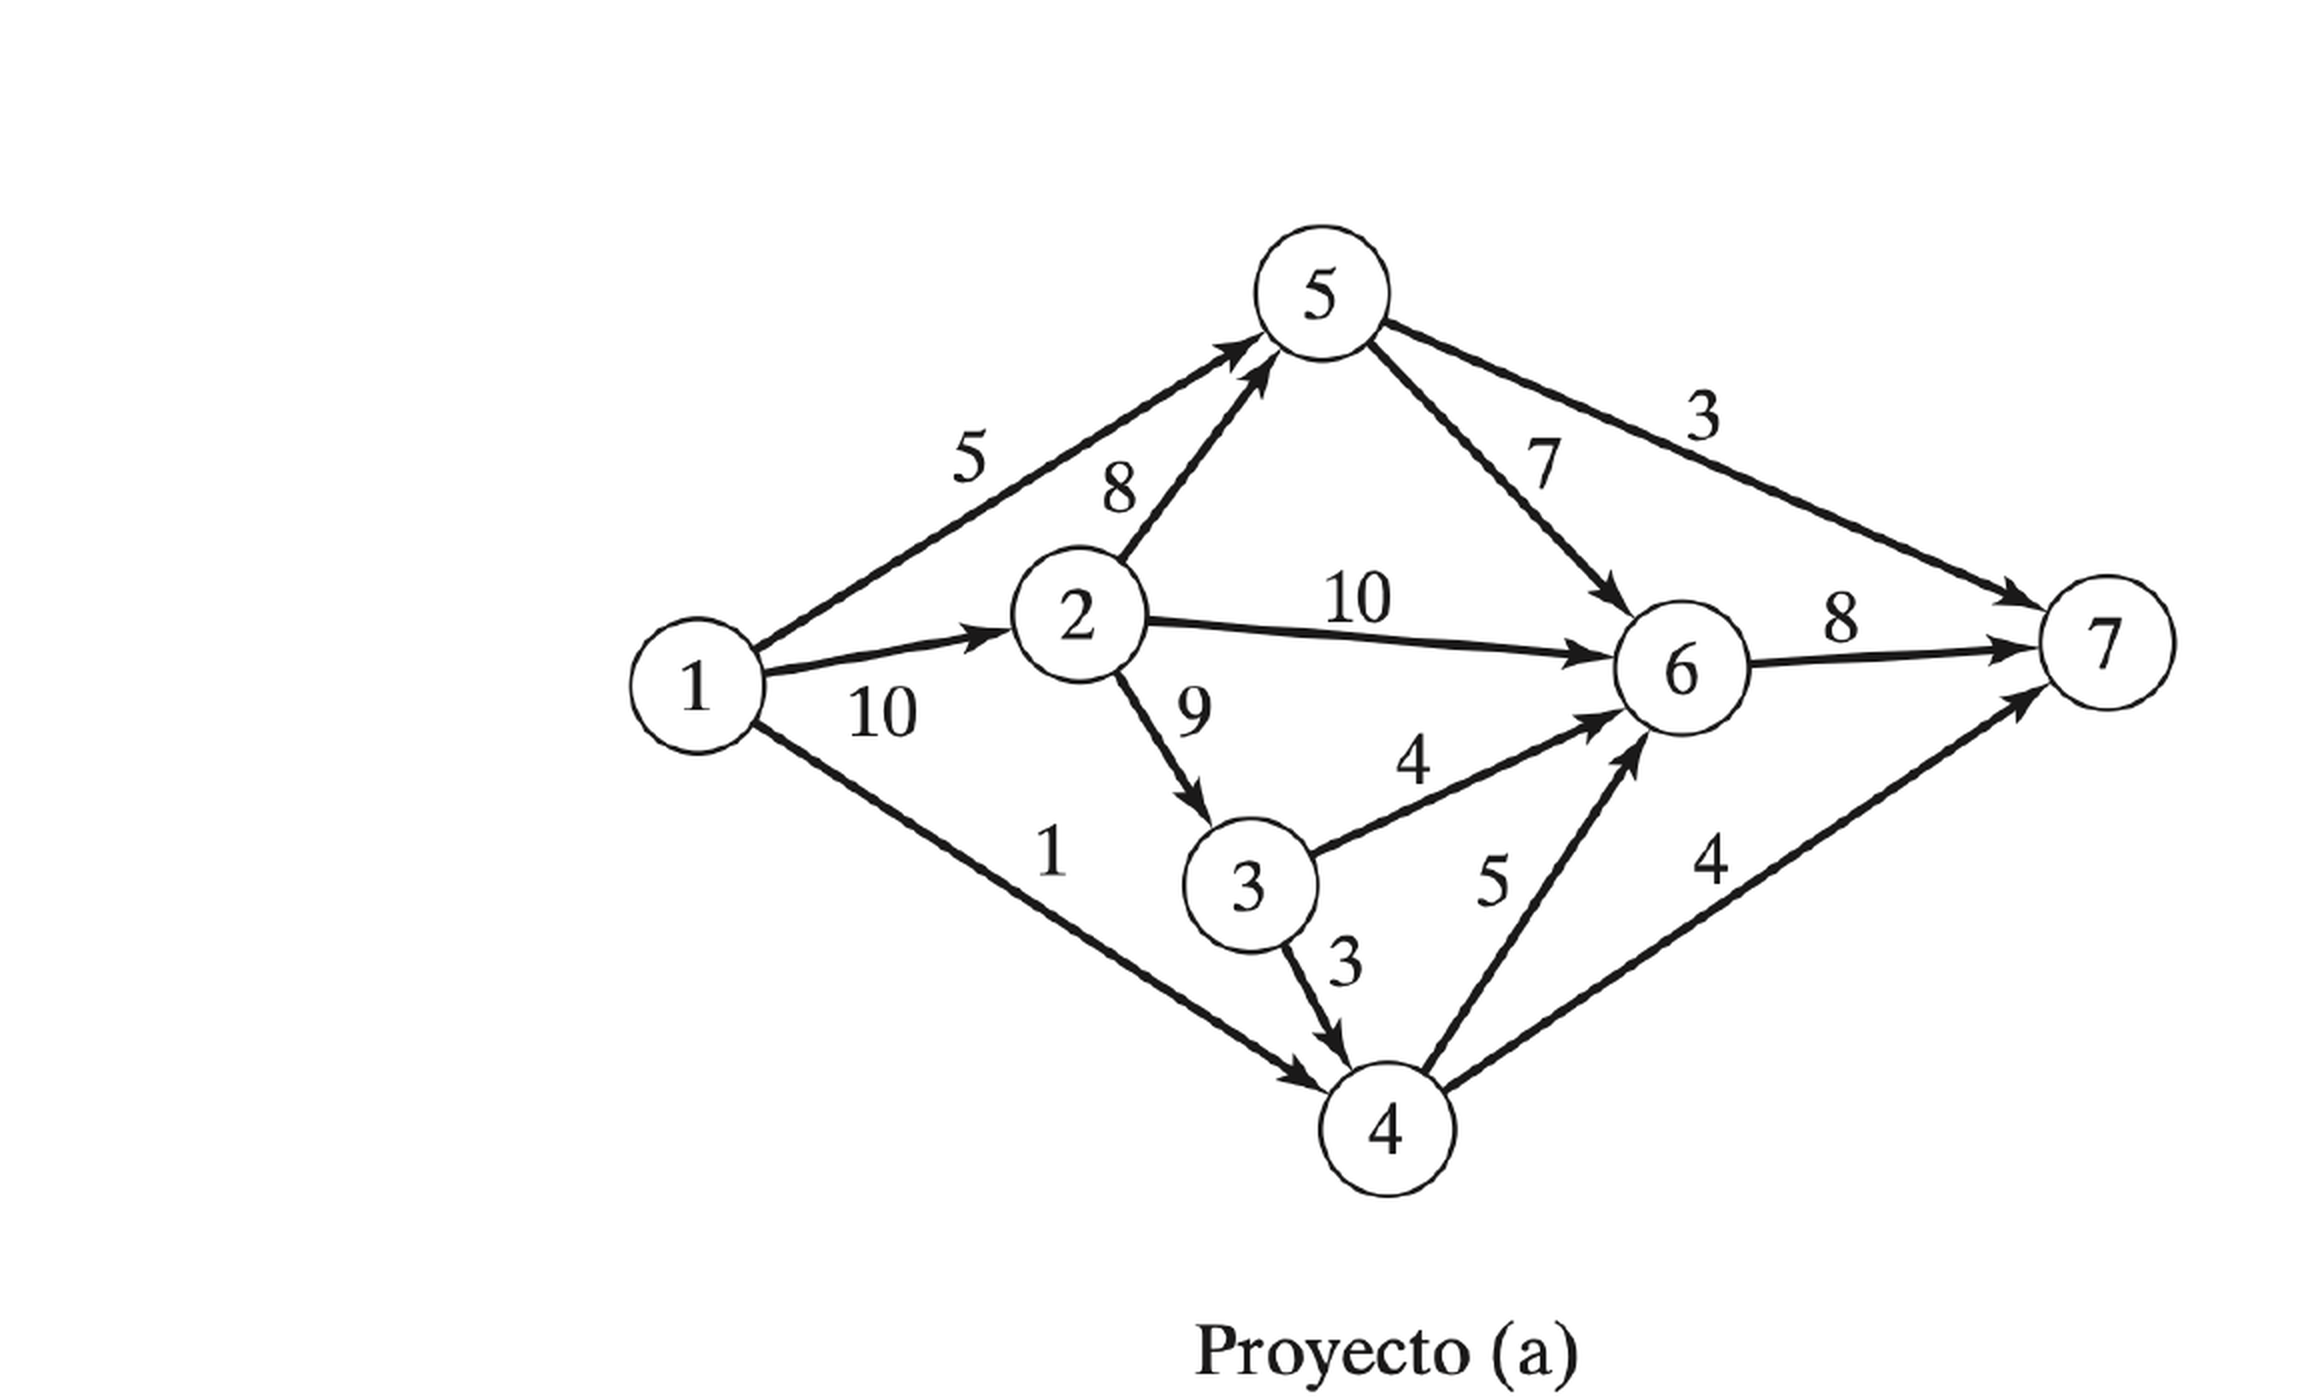
\includegraphics[width=0.9\textwidth]{imagenes/proyecto_a.png}
\caption{Red del Proyecto (a)}
\end{figure}

\begin{center}
\small
\begin{tabular}{|c|c|c|c|c|c|c|c|c|}
\hline
\textbf{Act.} & \textbf{Dur.} & \textbf{ES} & \textbf{EF} & \textbf{LS} & \textbf{LF} & \textbf{TF} & \textbf{FF} & \textbf{¿Crítica?} \\
\hline
1-2 & 10 & 0  & 10 & 0  & 10 & 0  & 0  & Sí \\
1-4 & 1  & 0  & 1  & 21 & 22 & 21 & 21 & No \\
1-5 & 5  & 0  & 5  & 15 & 20 & 15 & 13 & No \\
2-3 & 9  & 10 & 19 & 10 & 19 & 0  & 0  & Sí \\
2-5 & 8  & 10 & 18 & 12 & 20 & 2  & 0  & No \\
2-6 & 10 & 10 & 20 & 17 & 27 & 7  & 7  & No \\
3-4 & 3  & 19 & 22 & 19 & 22 & 0  & 0  & Sí \\
3-6 & 4  & 19 & 23 & 23 & 27 & 4  & 4  & No \\
4-6 & 5  & 22 & 27 & 22 & 27 & 0  & 0  & Sí \\
4-7 & 4  & 22 & 26 & 31 & 35 & 9  & 9  & No \\
5-6 & 7  & 18 & 25 & 20 & 27 & 2  & 2  & No \\
5-7 & 3  & 18 & 21 & 32 & 35 & 14 & 14 & No \\
6-7 & 8  & 27 & 35 & 27 & 35 & 0  & 0  & Sí \\
\hline
\end{tabular}
\end{center}

\textbf{Conclusión:} La duración total del proyecto (a) es $T=35$. La ruta crítica es única: $1\to2\to3\to4\to6\to7$ ($10+9+3+5+8=35$).

\begin{figure}[H]
\centering
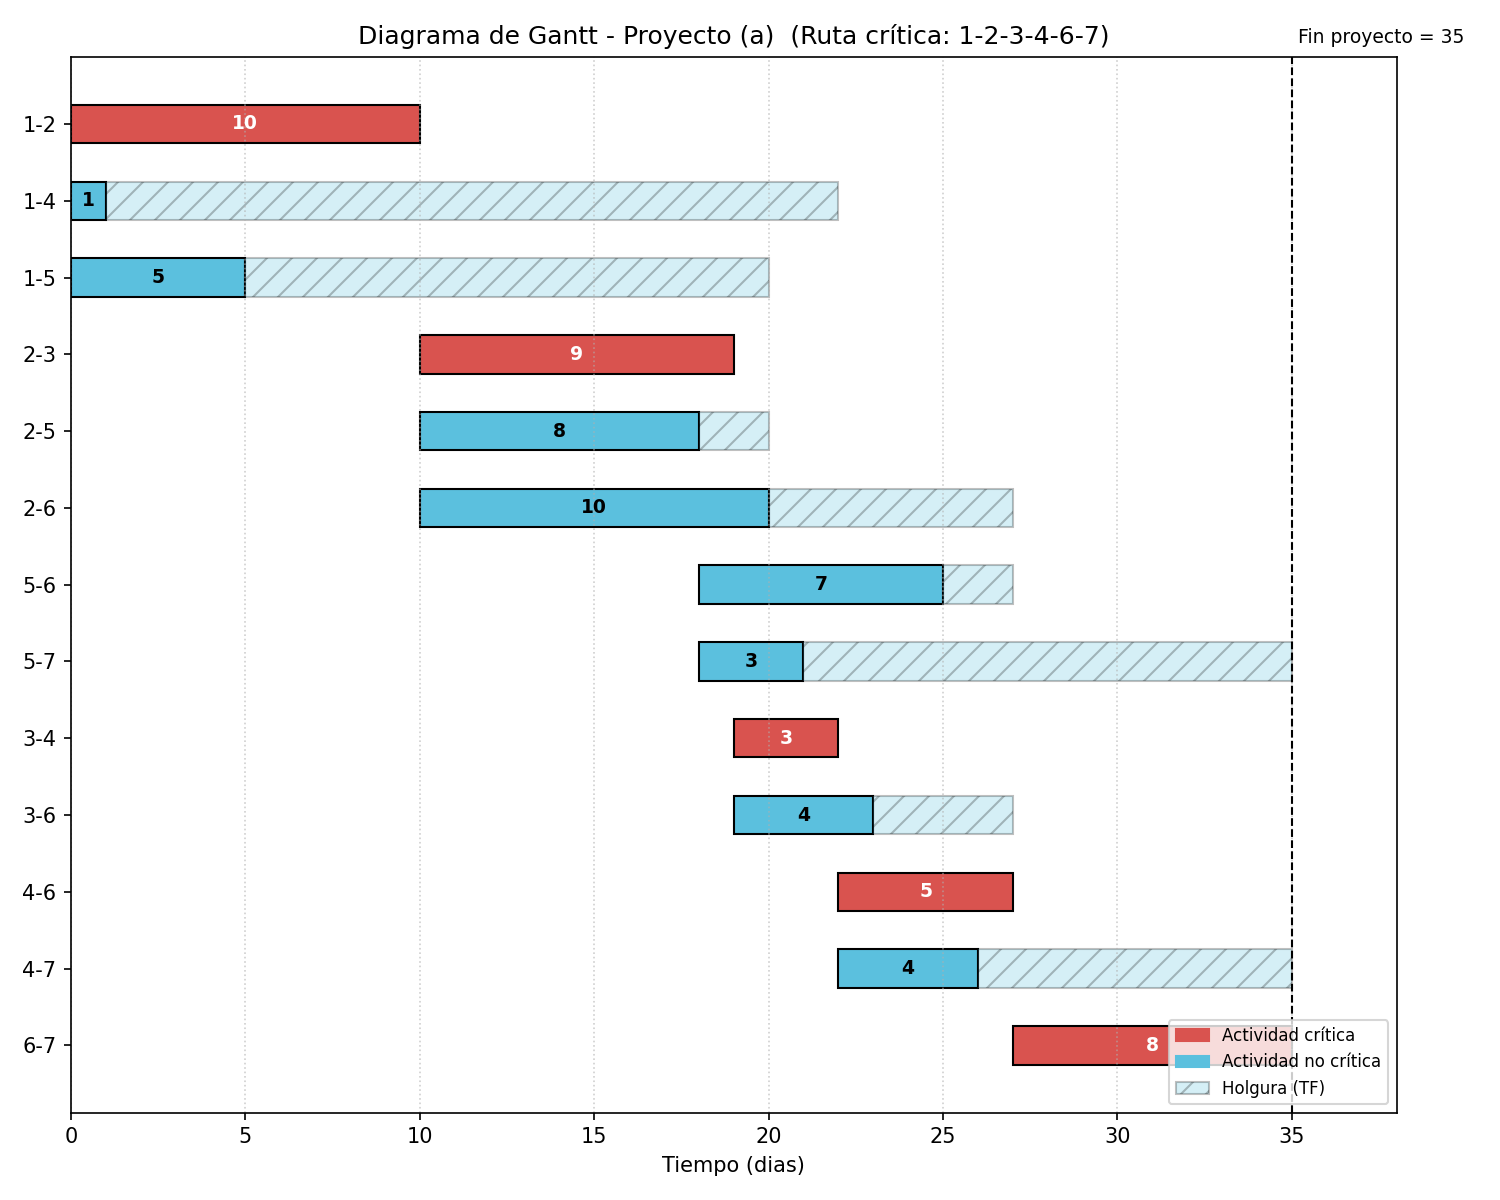
\includegraphics[width=0.85\textwidth]{imagenes/gantt_a.png}
\caption{Diagrama de Gantt -- Proyecto (a)}
\end{figure}

\clearpage
\medskip
\noindent\textbf{Proyecto (b)}\\

\begin{figure}[H]
\centering
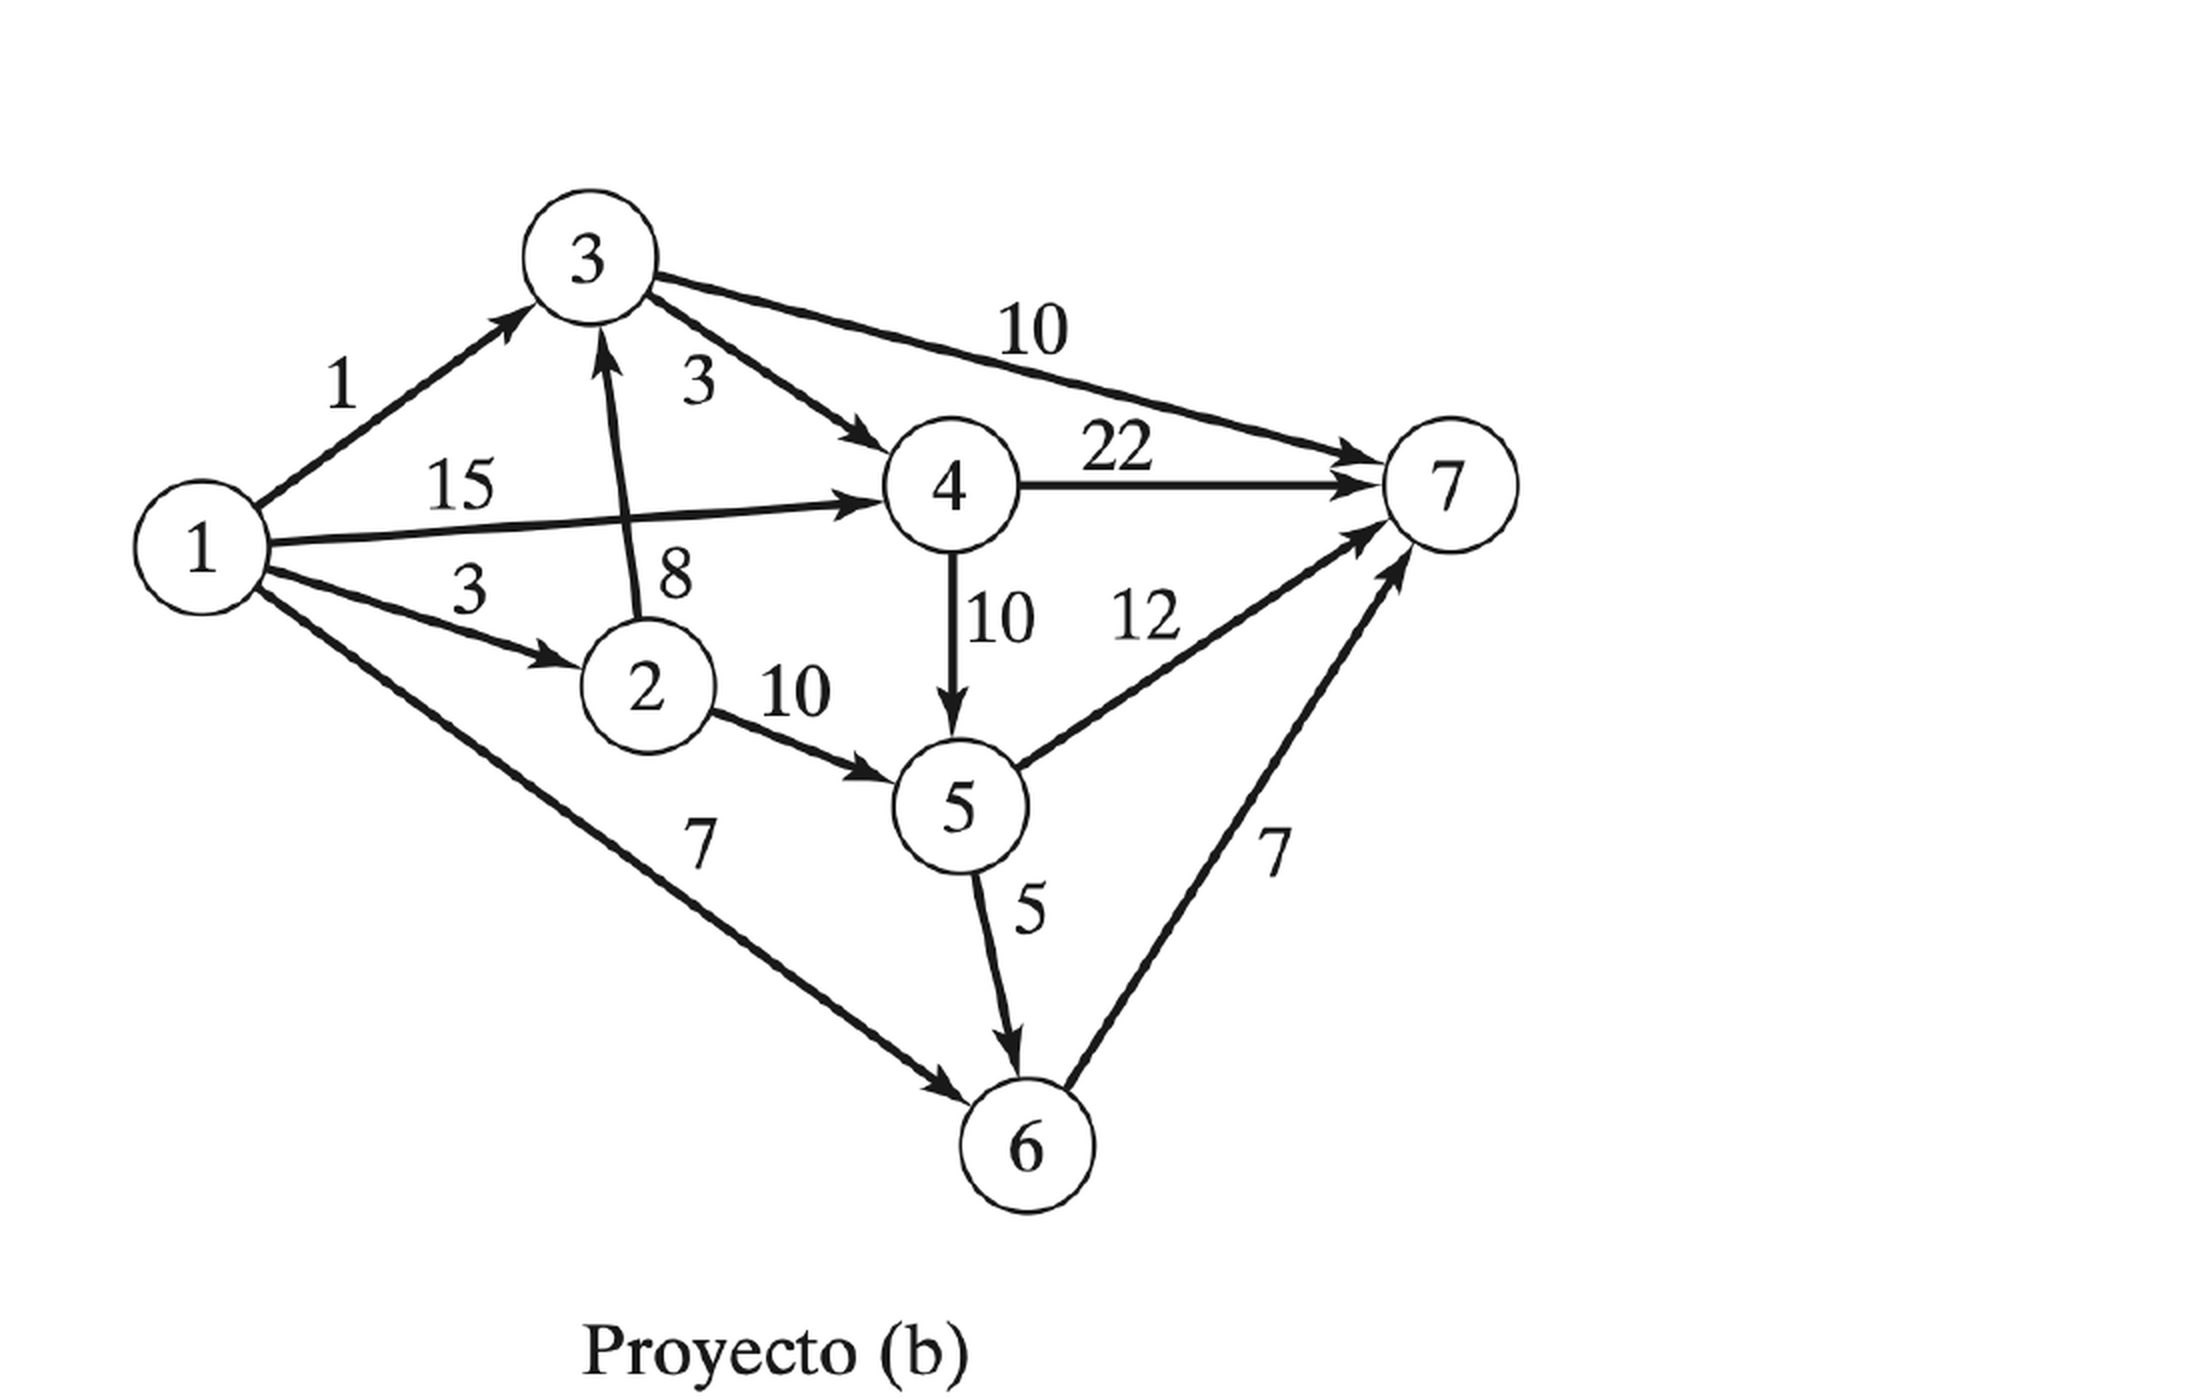
\includegraphics[width=0.9\textwidth]{imagenes/proyecto_b.png}
\caption{Red del Proyecto (b)}
\end{figure}

\begin{center}
\small
\begin{tabular}{|c|c|c|c|c|c|c|c|c|}
\hline
\textbf{Act.} & \textbf{Dur.} & \textbf{ES} & \textbf{EF} & \textbf{LS} & \textbf{LF} & \textbf{TF} & \textbf{FF} & \textbf{¿Crítica?} \\
\hline
1-2 & 3  & 0  & 3  & 1  & 4  & 1  & 0  & No \\
1-3 & 1  & 0  & 1  & 11 & 12 & 11 & 10 & No \\
1-4 & 15 & 0  & 15 & 0  & 15 & 0  & 0  & Sí \\
1-6 & 7  & 0  & 7  & 23 & 30 & 23 & 23 & No \\
2-3 & 8  & 3  & 11 & 4  & 12 & 1  & 0  & No \\
2-5 & 10 & 3  & 13 & 15 & 25 & 12 & 12 & No \\
3-4 & 3  & 11 & 14 & 12 & 15 & 1  & 1  & No \\
3-7 & 10 & 11 & 21 & 27 & 37 & 16 & 16 & No \\
4-5 & 10 & 15 & 25 & 15 & 25 & 0  & 0  & Sí \\
4-7 & 22 & 15 & 37 & 15 & 37 & 0  & 0  & Sí \\
5-6 & 5  & 25 & 30 & 25 & 30 & 0  & 0  & Sí \\
5-7 & 12 & 25 & 37 & 25 & 37 & 0  & 0  & Sí \\
6-7 & 7  & 30 & 37 & 30 & 37 & 0  & 0  & Sí \\
\hline
\end{tabular}
\end{center}

\textbf{Conclusión:} La duración total del proyecto (b) es $T=37$. A diferencia del Proyecto (a), aquí existe un \textbf{empate de tres rutas críticas}, debido a que $22 = 10+12 = 10+5+7$:
\begin{itemize}
    \item $1\to4\to5\to6\to7 = 15+10+5+7=37$
    \item $1\to4\to5\to7 = 15+10+12=37$
    \item $1\to4\to7 = 15+22=37$
\end{itemize}
Las actividades $1$-$4$, $4$-$5$, $4$-$7$, $5$-$6$ y $5$-$7$ son críticas ($TF=0$); el resto presenta holgura positiva.

\begin{figure}[H]
\centering
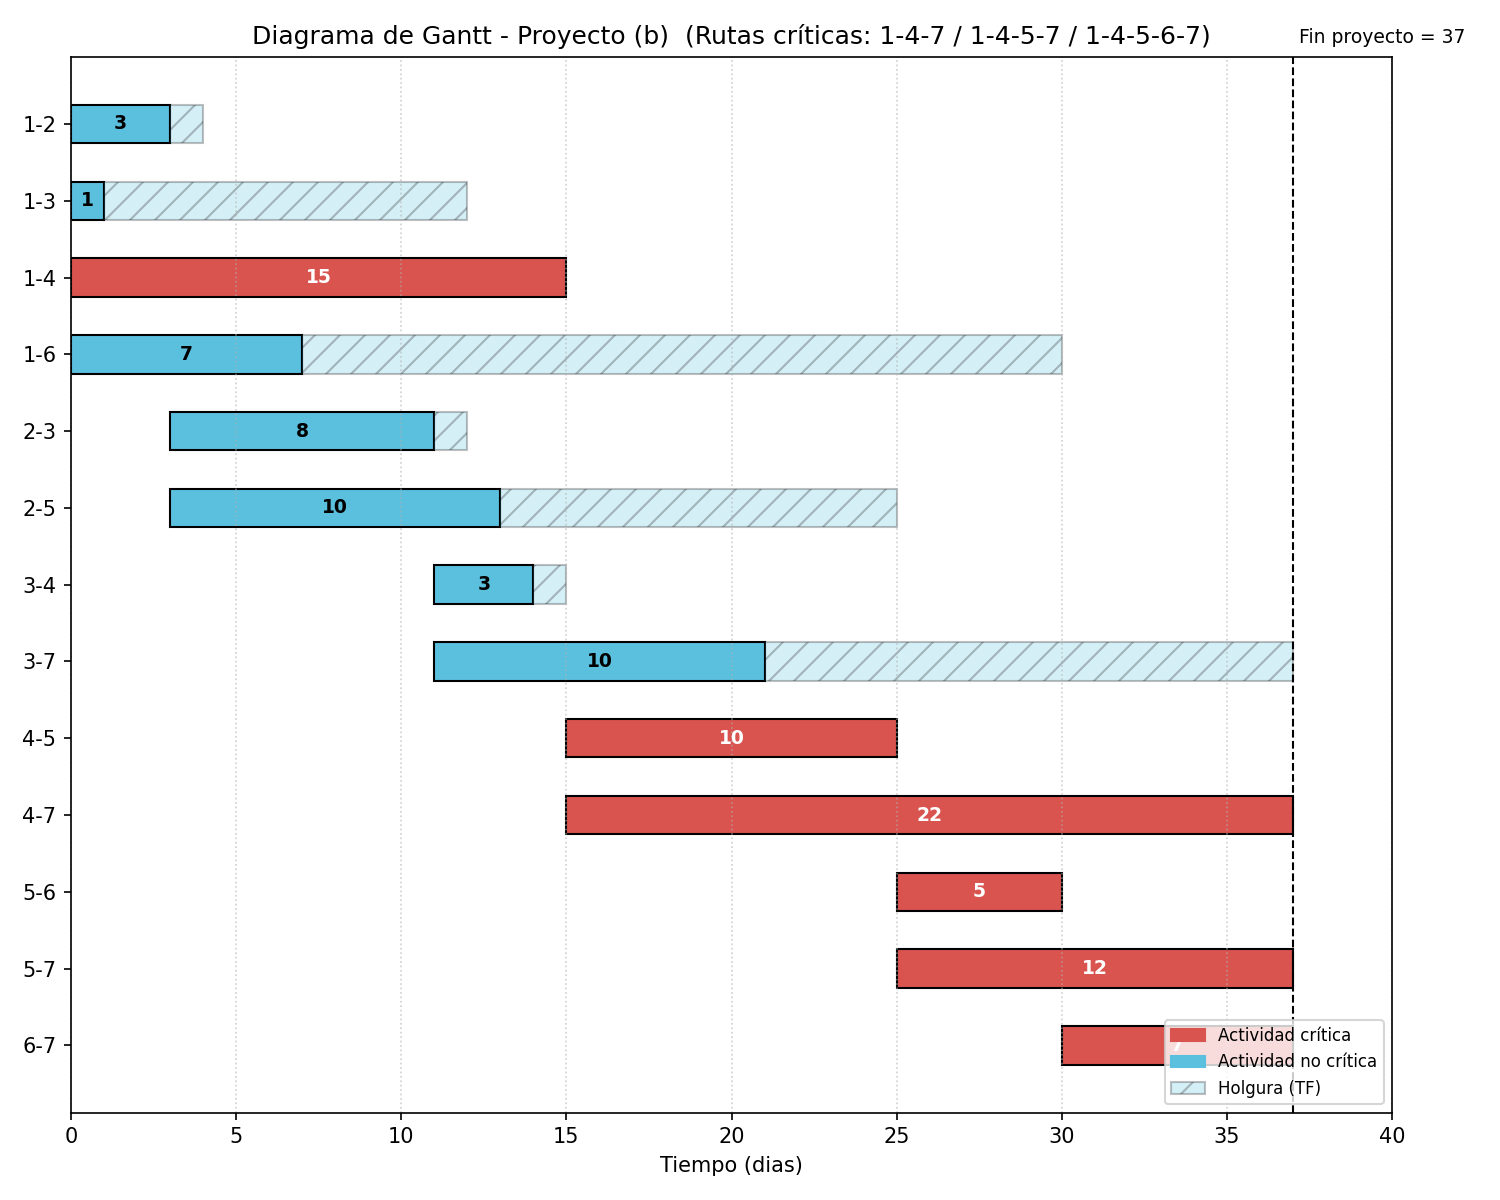
\includegraphics[width=0.85\textwidth]{imagenes/gantt_b.png}
\caption{Diagrama de Gantt -- Proyecto (b)}
\end{figure}

\clearpage
\subsection{Habilidades blandas empleadas en la práctica}

\begin{itemize}
    \item[$\boxtimes$] Liderazgo
    \item[$\boxtimes$] Trabajo en equipo
    \item[$\square$] Comunicación asertiva
    \item[$\square$] La empatía
    \item[$\boxtimes$] Pensamiento crítico
    \item[$\square$] Flexibilidad
    \item[$\square$] La resolución de conflictos
    \item[$\square$] Adaptabilidad
    \item[$\boxtimes$] Responsabilidad
\end{itemize}

\subsection{Conclusiones}

La aplicación del método CPM permitió determinar de forma sistemática los tiempos más tempranos y más tardíos de inicio y finalización de cada actividad, así como identificar las rutas críticas de los proyectos analizados. En el Ejercicio 2, la red de precedencias (AON) arrojó una duración total de 35 días, con la ruta crítica A--C--D--E--F--G y una única actividad no crítica (B, con $TF=FF=13$). En el Ejercicio 3 se demostró, tanto teórica como numéricamente, que toda actividad crítica posee holguras total y libre nulas ($TF=FF=0$), dado que $0 \le FF \le TF$. Finalmente, en el Ejercicio 5 se resolvieron dos redes AOA: el Proyecto (a), con una ruta crítica única ($1$-$2$-$3$-$4$-$6$-$7=35$), y el Proyecto (b), con un empate de tres rutas críticas ($T=37$), lo cual evidencia que un proyecto puede tener más de una secuencia de actividades igualmente determinante para su duración total. Los diagramas de Gantt elaborados permitieron visualizar de forma clara la programación de actividades y las holguras disponibles en cada caso.

\subsection{Recomendaciones}
Se recomienda revisar información complementaria sobre redes de proyectos y el método de la ruta crítica, idealmente contrastando los cálculos manuales con software especializado como MS Project, lo cual facilita la actualización de cronogramas ante cambios en las duraciones o precedencias. Asimismo, se sugiere mantener un control continuo de las holguras durante la ejecución del proyecto, pues una actividad no crítica puede convertirse en crítica si su retraso consume por completo su holgura disponible. Se recomienda además resolver ejercicios adicionales de redes con empates de rutas críticas, como el Proyecto (b) del Ejercicio 5, para afianzar la comprensión del concepto \cite{taha2017, pmi2017}.

\subsection{Referencias}

\vspace{-3em} %reduce el espacio causado por refname vacío
\renewcommand{\refname}{}
\bibliographystyle{ieeetr}
\bibliography{sample}


\end{document}
